\iffalse
It's unfair to say that mathematicians aren't real doctors, we perform surgeries all the time. In this class we'll introduce the notion of a topological manifold via simplicial (delta) complexes. Spend a day or two doing examples and go over several notions like orientation, cobordism and of course surgery.

Keywords: simplicial complex, manifold, orientation, cobordism, surgery

Type: Lecture
Homework: Recommended
Prereqs: None
\fi




\documentclass{article}
\usepackage{amsmath, amsthm}
\usepackage{amssymb}
\usepackage{mathtools}
\usepackage[all,cmtip]{xy}
\usepackage{color}


\setcounter{tocdepth}{4}

\renewenvironment{proof}{ {\bfseries Proof:}}{\qed}

\newtheoremstyle{mytheorem}%                % Name
{}%                                     % Space above
{}%                                     % Space below
{\itshape}%                                     % Body font
{0pt}%\parindent}%                                     % Indent amount
{\bfseries}%                            % Theorem head font
{.}%                                    % Punctuation after theorem head
{ }%                                    % Space after theorem head, ' ', or \newline
{}%                                     % Theorem head spec (can be left empty, meaning `normal')

\theoremstyle{mytheorem}
\newtheorem{thm}{Theorem}[section]
\newtheorem{proposition}[thm]{Proposition}
\newtheorem{lemma}[thm]{Lemma}
\newtheorem{corollary}[thm]{Corollary}


\newtheoremstyle{mydefinition}%                % Name
{}%                                     % Space above
{}%                                     % Space below
{}%                                     % Body font
{0pt}%\parindent}%                                     % Indent amount
{\bfseries}%                            % Theorem head font
{.}%                                    % Punctuation after theorem head
{ }%                                    % Space after theorem head, ' ', or \newline
{}%                                     % Theorem head spec (can be left empty, meaning `normal')

\theoremstyle{mydefinition}
\newtheorem{definition}[thm]{Definition}
\newtheorem{example}[thm]{Example}
\newtheorem{exercise}[thm]{Exercise}
\newtheorem{remark}[thm]{Remark}
%\newtheorem{ques}[thm]{Q.}
\newtheorem*{ques}{Question}
%\newtheorem{ans}[thm]{Ans.}
\newtheorem*{ans}{Ans}



\numberwithin{equation}{section}

%Real numbers, complex numbers, etc.
\newcommand{\R}{\mathbb{R}}
\newcommand{\C}{\mathbb{C}}
\newcommand{\Z}{\mathbb{Z}}
\newcommand{\Q}{\mathbb{Q}}
\renewcommand{\P}{\mathbb{P}}

%How does latex not have these?
\DeclareMathOperator{\Ad}{Ad}
\DeclareMathOperator{\ad}{ad}
\DeclareMathOperator{\tr}{tr}
\DeclareMathOperator{\Tr}{Tr}
\DeclareMathOperator{\Hom}{Hom}
\DeclareMathOperator{\Spec}{Spec}
\DeclareMathOperator{\im}{im}
\DeclareMathOperator{\rank}{rank}
\DeclareMathOperator{\Exists}{\exists}
\DeclareMathOperator{\Forall}{\forall}

\DeclareMathOperator*{\colim}{colim}
\DeclareMathOperator*{\holim}{holim}
\DeclareMathOperator*{\hocolim}{hocolim}


%fractions and inner product
\newcommand{\pr}[2][\:]{\frac{\partial #1}{\partial #2}}
\newcommand{\innerp}[2]{\langle #1, #2 \rangle}

\newcommand*\conj[1]{\overline{#1}}
\newcommand*\norm[1]{\lVert #1 \rVert}

\renewcommand{\figurename}{Fig.}
\usepackage{float}
\usepackage{wrapfig}

\usepackage{enumitem}
\setlist[enumerate]{itemsep=0mm}
\usepackage{geometry}
\geometry{
	a4paper,
	total={170mm,257mm},
	left=20mm,
	top=20mm
}


\usepackage{fancyhdr}
\pagestyle{fancy}
\lhead{\scshape Apurva Nakade}
%\rhead{\scshape Mathcamp 2017}
\renewcommand*{\thepage}{\small\arabic{page}}


\rhead{\scshape Mathcamp 2017 : All things Manifoldy}

\begin{document}
\title{Surfaces}
\author{Apurva Nakade}
\thispagestyle{fancy}
\maketitle



%%%%%%%%%%%%%%%%%%%%%%%%%%%%%%%%%%%%%%%%%%%%%%%%%%%%%%%%%%%%
%%%%%%%%%%%%%%%%%%%%%%%%%%%%%%%%%%%%%%%%%%%%%%%%%%%%%%%%%%%%
\section{Real projective space $\R\P^2$}
One way to define the projective plane is by gluing the antipodal points on the disc. In this section we'll see how this corresponds to lines in $\R^3$.

Consider the upper hemisphere
\begin{align*}
	S^2_+ = \{ (x,y,z) : x^2 + y^2 + z^2 = 1 , z\ge 0\}
\end{align*}
Every line in $\R^3$ intersects $S^2_+$ in exactly one point, unless the line is along the $x-y$ plane in which case it intersects $S^2_+$ boundary in antipodal points. Thus the set of lines in $\R^3$ is in 1-1 correspondence with the points on $S^2_+$ but with the antipodal points on the boundary circle glued, but this is precisely $\R\P^2$!

\begin{figure}[H]
	\centering
	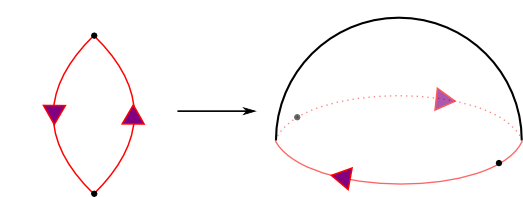
\includegraphics[width=0.25\linewidth]{images/ProjectivePlane}
	\caption{Real projective plane}
\end{figure}


\begin{exercise}
	Describe the space $\R\P^1$, the space of lines in $\R^2$.
\end{exercise}
%%%%%%%%%%%%%%%%%%%%%%%%%%%%%%%%%%%%%%%%%%%%%%%%%%%%%%%%%%%%
%%%%%%%%%%%%%%%%%%%%%%%%%%%%%%%%%%%%%%%%%%%%%%%%%%%%%%%%%%%%
\section{Poincar\'e conjecture}

Poincar\'e conjecture is perhaps the most celebrated conjecture in the theory of manifolds. It's solution(s) led to creation of a lot of amazing mathematics. For 3 dimensional manifolds the conjecture is as follows.

\begin{thm}[Poincar\'e conjecture]
	Let $M$ be a compact connected 3 dimensional manifold (without boundary). Suppose every loop on $M$ can be shrunk to a point then $M$ is homeomorphic to the 3 dimensional sphere $S^3$.
\end{thm}

There is a generalization of this conjecture to higher dimensions which requires a little more language to state. Surprisingly the conjecture was first proven to be true for dimensions $\ge 5$ by Smale, next for dimension 4 by Freedman and finally for dimension 3 by Perelman. The conjecture is \textbf{false} in the `category' of smooth manifolds i.e. if we replace homeomorphism by something stronger like diffeomorphism. The fact that the conjecture is true in the topological `category' but false in the smooth `category' implies the existence of \textbf{exotic manifolds}. Exotic spheres were first discovered by Milnor and only exist in dimensions 7 and higher. Freedman proved that $\R^4$ is the only Euclidean space which supports an exotic structure.

The Poincar\'e conjecture in dimension 2 follows from the classification theorem for surfaces.

\begin{thm}[Classification of surfaces]
	Every compact connected 2-dimensional manifold (without boundary) is homeomorphic to one of the following:
	\begin{enumerate}
		\item $S^2$
		\item $T^{\#k}$ for some $k$
		\item $(\R\P^2)^{\#k}$ for some $k$
	\end{enumerate}
\end{thm}

The Poincare conjecture for 2 dimensions is an easy consequence of this theorem.

\begin{exercise}
	Find a loop on each of the following spaces $T$, $\R\P^2$ and $K$ which cannot be shrunk to a point.
\end{exercise}

\begin{exercise}
	Show that for any compact connected manifold $M$ there is a loop in each of the spaces $M \# T$ and $M \# \R\P^2$ which cannot be shrunk to a point.
\end{exercise}

\begin{exercise}
	For a compact connected 2 dimensional manifold $M$ (without boundary) show that if every loop on $M$ can be shrunk to a point then $M$ is homeomorphic to $S^2$.
\end{exercise}












\iffalse
A two dimensional manifold is called a surface. The surface of the earth is an example of a two dimensional manifold. By the above definition a surface is set $S$ such every point $s \in S$ has a neighborhood homeomorphism to a 2 dimensional disk.

\begin{figure}[H]
	\centering 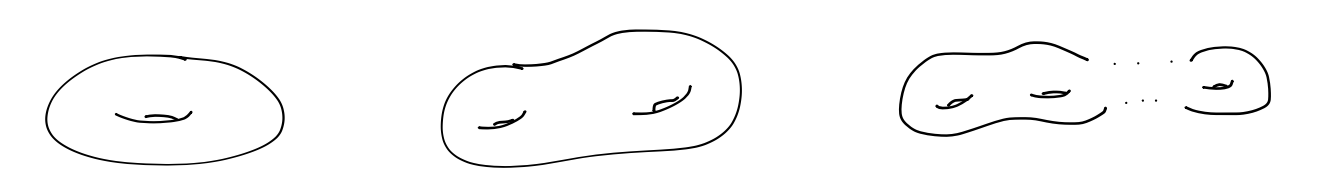
\includegraphics[width=0.85\linewidth]{images/GegusGSurfaces}
	\caption{Surfaces}
\end{figure}

\subsection{Connected sums}
It is not hard to see that we can make sense of `addition' of two surfaces, after all when we think of a genus $g$ surface we think of $g$ tori glued to each other.

If $M_1$ and $M_2$ are two surfaces of genus $g_1$ and $g_2$ then we can `add' $M_1$ and $M_2$ to get a surface of genus $g_1+ g_2$. This is done by removing a small disc from $M_1$ and $M_2$ each and gluing $M_1$ and $M_2$ along the holes. The resulting manifold is denoted by $M_1 \# M_2$ and is called their \textbf{connected sum}.

We will denote a torus by $T$ and a genus $g$ surface by $T \# \cdots \# T$, $g$ times or simply as $T^{\#g}$.

\begin{figure}[h]
	\centering \includegraphics[width=0.40\linewidth]{images/ConnectedSum}
	\caption{Connected sum}
\end{figure}

Thus it is possible to add two surfaces but not subtract them. There is also an \emph{identity element} for this connected sum operation (what is it?). This is more formally expressed by saying that the set of surfaces (up to homeomorphism) is a \textbf{monoid}.

\begin{exercise}
	Define connected sum for arbitrary manifolds.
\end{exercise}

\begin{exercise}
	In the definition of connected sum we removed arbitrary discs from the manifolds $M_1$ and $M_2$. Draw pictures to show that if any two such choices can be deformed into each other and hence up to homeomorphism the manifold $M_1 \# M_2$ is well defined. Can you come up with a rigorous proof for this?
\end{exercise}

\begin{ques}
	Is every surface a genus $g$ surface for some integer $g$?
\end{ques}
The answer is no. The most famous example is perhaps the Klein bottle. The Klein bottle is an example of a non-orientable surface (a surface with only 1 side) and it cannot be embedded in $\R^3$.
\begin{figure}[H]
	\centering
	\includegraphics[width=0.15\linewidth]{images/KleinBottle}
	\caption{Klein bottle}
\end{figure}

There is an amazing theorem that holds for 2 dimensional manifold but which does not hold in any higher dimension.

\begin{thm}[Classification of surfaces]
	Every compact connected 2 dimensional manifold is homeomorphic to one of the following
	\begin{enumerate}
		\item $S^2$
		\item $T^{\#g}$
		\item $(\R\P^2)^{\#g}$
	\end{enumerate}
\end{thm}
We'll define the surface $\R\P^2$, called the \textbf{real projective plane} below. If we think of a 2 dimensional manifold sitting inside some $\R^n$ then \textbf{compact connected} means that as a set the manifold is \textbf{closed} and \textbf{bounded}. If you do not know what these words mean then intuitively compact connected means that the manifold has no punctures in it and it does not extend to infinity.

How might one try to prove such a theorem? We'll use a technique very popular in topology called cutting and pasting!

\subsection{Gluing diagrams}
\begin{ques}
	What does a connected sum of a Klein bottle and a torus give us? What is the connected sum of two Klein bottles?
\end{ques}

To answer the above question we try to covert the problem into combinatorics by cutting open the surface. If cut a torus once we get a cylinder and we cut the cylinder again we get a square. On the square we label the sides to remember which side should be glued to which to get back the torus. Such a diagram is called a \textbf{gluing diagram}.

\begin{figure}[H]
	\centering
	\includegraphics[width=0.20\linewidth]{images/GluingDiagramTorus}
	\caption{Gluing diagram for a torus}
\end{figure}

Can we find gluing diagrams for other surfaces? The connected sum comes to the rescue. We can use connected sums to construct gluing diagrams using $2g$ sided polygons to construct $g$ genus surfaces, as in figure \eqref{ConnectedSumGluingDiagram}.

\begin{figure}[h]
	\centering
	\includegraphics[width=0.50\linewidth]{images/GluingDiagramConnectedSum1}
	\includegraphics[width=0.60\linewidth]{images/GluingDiagramConnectedSum2}
	\caption{Connected sum and gluing diagrams}
	\label{ConnectedSumGluingDiagram}
\end{figure}

This is an interesting development. Perhaps we can even find a gluing diagram for the Klein bottle. What happens when you cut open the Klein bottle?

\begin{figure}[H]
	\centering
	\includegraphics[width=0.20\linewidth]{images/GluingDiagramKleinBottle}
	\caption{Gluing diagram for a Klein bottle}
\end{figure}

\begin{ques}
	What happens if we do not put arrows on all the edges?
\end{ques}

\begin{ques}
	What do open sets and line segments look like on the gluing diagrams?
\end{ques}

\begin{ques}
	When does the gluing diagram give us a manifold?
\end{ques}

\begin{ques}
	Can you come up with a gluing diagram for a sphere?
\end{ques}

%%%%%%%%%%%%%%%%%%%%%%%%%%%%%%%%%%%%%%%%%%%%%
%%%%%%%%%%%%%%%%%%%%%%%%%%%%%%%%%%%%%%%%%%%%%
\subsection{Classifying surfaces}
Notice that if we flip the directions of both the arrows labelled $a$ on the gluing diagram for a torus we get the torus back, but if we flip only one of the $a$ while keeping the other fixed we get a Klein bottle. This begs the question,

\begin{ques}
	What happens when we flip both the arrows on the torus gluing diagram?
\end{ques}
This gives us the \textbf{Projective plane} denoted by $\R\P^2$. This is the space that we encountered in the classification theorem.
\begin{figure}[H]
	\centering
	\includegraphics[width=0.20\linewidth]{images/GluingDiagramProjectivePlane}
	\caption{Gluing diagram for the Projective Plane $\R\P^2$}
\end{figure}

The proof of the classification theorem has two main steps. First comes from point set topology. First we show that any compact connected surface gives rise to a gluing diagram. This is a highly non-trivial fact that we will assume. The proof of this requires some knowledge of the fundamental group.

The second step is the showing that any gluing diagram is of one of three types listed in the classification theorem.

\subsection{The algebra of gluing diagrams}
We saw how connected sums allowed us to construct gluing diagrams for genus $g$ surfaces. A connected sum is a cutting and pasting operation. We can do more interesting cutting and pasting operations and produce some non-trivial results about gluing diagrams.

\begin{figure}[h]
	\centering
	\includegraphics[width=0.75\linewidth]{images/GluingDiagramKleinBottleMobiusStrip}
	\caption{Klein bottle is the connected sum of two Mobius strips}
\end{figure}
\fi
\end{document}









%%%%%%%%%%%%%%%%%%%%%%%%%%%%%%%%%%%%%%%%%%%%%%%%%%%%%%%%%%%%
%%%%%%%%%%%%%%%%%%%%%%%%%%%%%%%%%%%%%%%%%%%%%%%%%%%%%%%%%%%%
\section{Modular origami}

\subsection{Orientation of surfaces}
Let us start with surfaces. Roughly speaking a surface is called orientable if has two sides. A sphere or a torus are easily seen to be orientable. In fact any surface that can be \textit{embedded} in $\R^3$ is orientable. A Mobius strip on the other hand (which is not a surface as it has a boundary) is not orientable. With a little more mental effort one might be able to see that a Klein bottle or a Projective space are not orientable. We want an equivalent definition which can be used on gluing diagrams.

We begin by defining orientation of a polygon. An \textbf{orientation of a polygon} is simply a cyclic ordering of it's vertices. For example this is one of the two possible ways to orient a triangle with vertices $(0,1,2)$.

\begin{center}
	\begin{tabular}{c}
		\centering 
\includegraphics[height=3cm]{../noImageAvailable}
	\end{tabular}
\end{center}

\begin{exercise}
	This is related to the fact that the polygon has two sides via the right hand rule in physics. Do you see the connection?
\end{exercise}

An \textbf{orientation} of (a gluing diagram of) a surface is a compatible choice of orientation for each triangle, where the orientations of two adjacent triangles need to be compatible in the following way,
\begin{center}
	\begin{tabular}{c c c}
		\centering 
\includegraphics[height=3cm]{../noImageAvailable} & \: & \centering 
\includegraphics[height=3cm]{../noImageAvailable}
	\end{tabular}
\end{center}
This forces an edge to be directed in two different directions in adjacent triangles.

\begin{exercise}
	Add the diagonals to the standard gluing diagrams to obtain triangulations and try to find orientations for them. Conclude that $S^2,T$ are orientable and $\R\P^2,K$ are not.
\end{exercise}

\begin{exercise}
	Use gluing diagrams to show that $T\#T$ is orientable. Generalize this to argue that $T ^{\# n}$ are orientable.
\end{exercise}

This same method also allows us to understand manifolds in higher dimensions as well.







\subsection{Simplices}
As we go to higher dimensions polygons (or is it polytopes?) become whacky are themselves quite hard to understand. So instead of looking at arbitrary polygons we look at the simplest polygons: triangles. We'll upgrade the definition of a triangle to a simplex which can live in arbitrary dimensions.

\begin{definition}
	An $n$ dimensional \textbf{simplex} $\Delta^n$ is any set which is homeomorphic to the following region in $\R^{n}$.
	\begin{align}
		\{ (x_0, x_1, \cdots, x_n) : x_0 + \cdots + x_n \le 1 \mbox{ and each } x_i \ge 0  \}
	\end{align}
\end{definition}
A 1 dimensional simplex is a segment and a 2 dimensional simplex is a triangle.
Simplices are topologists best friend.

Note that by adding extra diagonal lines we could have made the gluing diagrams entirely out of triangles.
We represent a simplex by its set of vertices.

\begin{figure}[h]
	\centering 
\includegraphics{../noImageAvailable}
	\caption{Gluing diagram with labeled simplices}
	\label{}
\end{figure}

As with origami you can glue these simplices any way you want and get relaly interesting objects. We're going to glue them to create manifolds.

\subsection{Manifolds from simplices}
A delta complex is a collection of simplices glued along the faces.

\begin{definition}
	Faces of a simplex followed by examples.
\end{definition}

\begin{definition}
	Definition of a delta complex followed by several examples.
\end{definition}

Talk about spheres, tori and projective spaces in 3 dimensions.

\begin{ques}
	When is a delta complex a manifold?
\end{ques}

Examples of manifolds and non-manifolds.






%%%%%%%%%%%%%%%%%%%%%%%%%%%%%%%%%%%%%%%%%%%%%%%%%%%%%%%%%%%%
%%%%%%%%%%%%%%%%%%%%%%%%%%%%%%%%%%%%%%%%%%%%%%%%%%%%%%%%%%%%
\section{More on manifolds}
The last day is a little more on the expository side.

We saw how a Dehn surgery can be used to simplify a knot on a torus. We also saw how a connected sum can be used to build higher genus surfaces out of simpler ones.

Is it possible to simply go the other way? Can one reverse the connected sum operation and go from a more complicated manifold to a simple one?

\subsection{Orientation of manifolds}

Show that $\R\P^1$ and $\R \P^3$ are orientable but $\R\P^2$ is not using Delta complexes.

\subsection{Cutting $S^3$ into tori}

\subsection{Using Dehn twists to create 3 manifolds}




\end{document}
